\documentclass[12pt]{report}
\usepackage[a4paper, left=1in, right=1in, top=1in, bottom=1in]{geometry}
\usepackage{xcolor}
\usepackage{amsmath}
\usepackage{amsthm}
\usepackage{amssymb}
\usepackage{amsfonts}
\usepackage{algpseudocode}
\usepackage{mathtools}
\usepackage{xcolor}
\usepackage{float}
\usepackage{framed}
\usepackage{listings}
\usepackage{graphicx}
\usepackage{subcaption}
\usepackage{tikz}
\usepackage{emoji}

\lstset{basicstyle=\ttfamily,
  commentstyle=\color{red},
  keywordstyle=\color{blue},
  %basicstyle=\footnotesize,
  frame=lines,
  numbers=left,
  stepnumber=1,
  showstringspaces=false,
  tabsize=1,
  breaklines=true,
  breakatwhitespace=false,
}
\usepackage{hyperref}
\hypersetup
{
    colorlinks=true,
    linkcolor=blue,
    filecolor=magenta,
    urlcolor=cyan,
    pdftitle={\Huge \textbf{CS218 Solutions GreedyDP}},
    pdfpagemode=FullScreen,
}
\usepackage[utf8]{inputenc}
\usepackage{graphicx}
\usepackage{longtable}
\usepackage{multirow}
\usepackage{enumitem}
\setlength{\parindent}{0pt}

\begin{document}
\subsection*{\Large\bfseries Greedy Algorithms}
\begin{enumerate}[label=\textbf{\arabic*.}]

  \item Assuming there's a minimum weight spanning tree. It must have at least 1 edge in $C$, as the vertices in $V_1$ and $V_2$ have to be connected.
  If the edge $e^*$ is already in the spanning tree, we're done, so assume it's not there. Now add $e^*$, since we have too many edges, we'll have a cycle.
  We can also say that the cycle contains $e^*$, as that's the edge which when added, created a cycle. There must be some other edge in $C$ which is part of 
  the cycle. This is because is we walk through the cycle, we traverse $e^*$, moving from $V_1$ to $V_2$, so we must come back from $V_2$ to $V_1$, and that
  requires another edge in the cut. So now we can delete this other edge in the cut, and we get a spanning tree again, and this tree will have weight $\leq$
  the old tree, as $e^*$ was the minimum weight edge in the cut.

  \item Again, let's assume that we have a minimum spanning tree without $e^*$, and now add $e^*$. There will now be a cycle, and this cycle will contain 
  $e^*$. There must be another edge of this cycle containing $v_1$, as every vertex in a cycle must have 2 edges in the cycle. Now if we delete this other 
  edge, we will have a spanning tree, and this spanning tree will be minimum.

  \item Strategy 1 fails in cases where you actually have less time for larger assignments. Take an example there $l_1, l_2 = 1, 2$ and $d_1, d_2 = 3, 2$. If 
  you do 1 before 2, you finish 2 late, but if you do 1 after 2, you finish both on time.

  Strategy 3 seems logical. The reason we are using $d_i - l_i$ as a factor, is because that's the time remaining after we finish the assignment. So it's an 
  increasing order of how much extra time we will have for an assignment if we start now. But it can prioritize very long assignments over short ones which 
  need to be finished early. Take $l_1, l_2 = 1, 3$ and $d_1, d_2 = 3, 4$. Our greedy approach will make us do assignment 2 first, which makes us finish
  assignment 1 late. But if we did assignment 1 first, we would have enough time for assignment 2 after it.

  Now to prove the claim in strategy 2.
  Let's say $A_j$ is immediately done before $A_i$, but $A_j$ has a closer deadline compared to $A_i$. What happens if we swap $A_i$ and $A_j$? Firstly, it's
  clear that the lateness of any assignment other than $A_i$ and $A_j$ don't change. Now let's just look at $A_i$ and $A_j$. We can take cases, but I'll provide
  some sort of general reasoning as to why the swap won't decrease the max lateness.

  Before the swap, $A_j$ was finished later, but had an earlier deadline. So no matter what, the lateness will be more than or equal to $A_i$. So after swapping, 
  we just have to make sure the lateness of both $A_i, A_j$ are less than the lateness of $A_j$ before swapping. Firstly after swapping the lateness of $A_j$
  obviously decreases, it's done earlier. But the lateness of $A_i$ has increased. But think about it like this, $A_i$'s finishing time after swapping is same 
  as $A_j$'s finishing time before swapping. And also, $A_i$'s deadline is further away than $A_j$'s deadline. So since the finishing times are equal and we have 
  more time in 1 case, $A_i$'s lateness after swapping is $\leq$ $A_j$'s lateness before swapping.

  Now we can use this swapping trick to do the whole question. Assume there's an optimal solution which isn't increasing order of deadlines. We can just do an
  insertion sort like algorithm. And keep doing swaps to bring the array to increasing order of deadlines. We have also shown that in each swap, the max lateness
  isn't increasing, and it can't really decrease as we started with an optimal solution. So at the end of our insertion sort, the max lateness is same as that of
  the optimal solution, so increasing order of deadlines is always optimal.
  
  \item Since each assignment takes unit time, there's a simple way to check if an assignments is done on time. If you do the assignments in order, the $k^{th}$
  assignment is done on time if and only if its deadline is greater than or equal to $k$. We just now have to order the $n$ assignments, maximizing the total 
  reward.

  Here's how our greedy algorithm is going to work. We first sort the assignments in decreasing order of rewards. After that, assume the assignments are $A_1, 
  \dots, A_n$. Now we iterate through this array. We check if $A_i$ can be completed in time i.e. there's some empty spot from 1 to deadline of $A_i$. If there 
  is, we place in the last spot that we could, such that $A_i$ is completed in time. If not, we just place $A_i$ at the end of the array, or as far as possible 
  to the end.

  The algorithm is simple enough, but why does this work? We'll prove by induction that there is an optimal solution where $A_1, \dots, A_k$ are placed at the 
  same place as our algorithm. Let's explain how the induction works. Assume there's a solution where $A_1, \dots, A_{k-1}$ have been placed how they have in our 
  algorithm, now think about $A_k$.

  \begin{itemize}
    \item Case 1: There's a spot for $A_k$ such that it can be completed on time. Can we show that it's also completed on time in the optimal solution? If 
    not, in the optimal solution, there's some $A_l$ in the spot where $l > k$. But then just swap $A_l$ and $A_k$, now we get an extra reward due to $A_k$,
    we might lose the reward $A_l$. But our net gain is positive as reward of $A_k$ is more than reward of $A_l$. Now we have to show there's a solution 
    where it's placed as late as possible, but this is intuitive right. If it's placed eariler, just swap it with $A_l$ (whatever's in the latest spot), 
    $A_k$ is still completed, you still get its reward, and $A_l$ is completed even earlier, so it won't lose its reward either.

    \item Case 2: There's no spot for $A_k$ such that it can be completed on time. This would mean even in our optimal solution, $A_k$ isn't completed as there
    is literally no place for it to go. There is obviously some optimal solution where it's placed as late as possible, right. If it's placed earlier than that,
    just move it later, anyway it wasn't going to be completed on time, and you are moving some other assignment earlier, which definitely won't hurt.
  \end{itemize}

  \item This is actually a hard problem :/
  
  It's not really mentioned whether we can split up the time when we do a particular assignment, or that we have to do it in 1 whole stretch. But we can 
  see that it doesn't matter, actually splitting up assignments doesn't really help us. Let's say we are finishing some set of assignments $A_1$ to $A_n$, by 
  splitting them up. WLOG let's also assume the final finishing times of $A_1$ to $A_n$ are in ascending order. We claim that if we just did $A_1$ fully, then 
  $A_2$ fully, $\dots$, then $A_n$ fully, we would have accomplished the same thing. We can prove this by induction. We know $A_n$ is finished at the end, so
  it is finally finished at time $l(A_1) + l(A_2) + \dots + l(A_n)$ (where $l(A_i)$ is total length/time taken for assignment $A_i$). But why not rearrange the 
  time intervals, and do $A_n$ at the end? To be clear, we are picking out times whenever $A_n$ is done, and placing them at the end. The final time $A_n$ is 
  finishing at is still the same. And time intervals of the other assignments are moved earlier anyway, by this swapping. Now just do this for $A_{n-1}, A{n-2}$,
  so on until all of them are just done at a stretch.

  Now that we've proved this, let's just assume we can split up assignments. Now our greedy algorithm is going to work like this: first sort in increasing order of 
  assignment lengths. Now we iterate over the array, and check if the assignment $A_i$ can be completed in time i.e. there is at least $l(A_i)$ space before the 
  deadline of $A_i$. If so, we do $A_i$ as late as possible, and split it up to achieve this, if required. If it's not possible to do it on time, we just skip it.

  We now prove by induction: there exists an optimal solution where $A_1, \dots, A_k$ are finally finished at the same time as whenever our algo decides when they 
  should finish.

  Our inductive assumption: assume there's an optimal solution where $A_1, \dots, A_{k-1}$ are placed where they are. Now if there's enough empty space before deadline
  of $A_k$, we claim that there's an optimal solution where $A_k$ is done before the deadline. As most greedy questions, we assume there's an optimal solution without 
  $A_k$, and try to modify it such that $A_k$ is done too. Ok, our optimal solution doesn't actually do $A_k$ but it most likely does something else in the time when 
  it could have done $A_k$. Maybe it spent 1 unit of time on many assignments, maybe it did half of $A_{k+1}$, maybe it did nothing, we don't really know. But our idea 
  is to replace something with $A_k$ right, but we can't really do this if only partial assignments are done. If somehow a full assignment $A_l$ was done, we could have 
  replaced it with $A_k$, as $A_k$ takes lesser time than $A_l$ for all $l > k$. So what do we do? The insight now is to reorder intervals such that assignments are done 
  one by one, but we reorder only $A_{k+1}$, $A_{k+2}$, all the way to $A_n$.

  Let me explain what this reordering is exactly. Say $A_i$ was done in $[0,1]$, nothing was done in $[1,2]$, $A_j$ was done in $[2,3]$ and $A_i$ was done in $[3,4]$.
  We reorder such that no assignment is done between the starting and completion of another assignment, but importantly, we keep empty intervals empty. So if we want 
  to reorder in the example given, we do $A_j$ from $[0,1]$, nothing from $[1,2]$, $A_i$ from $[2,3]$ and $A_i$ from $[3,4]$.

  Ok, now after this reordering, now what do we see done before $A_k$'s deadline (other than $A_1$ to $A_{k-1}$). If suppose one of the assignments from $A_{k+1}$ to 
  $A_n$ was finished completely before $A_k$'s deadline, great. We just delete it and insert $A_k$. Now if none of these assignments were finished before $A_k$'s deadline,
  we can say only at most one of them was started before $A_k$'s deadline. Because, if one of them was started, it has to be completed before the next one is started, and
  none of them finish before $A_k$'s deadline. So what we can do is just delete this assignment. We'll now have enough empty intervals before the deadline of $A_k$
  to fit the length of $A_k$, move them to the end, and fit $A_k$.

  Now that we've proven there is an optimal solution with $A_k$, we have to show that $A_k$ is done as late as possible (just like how it's done in our algo). 
  But this is easy right, if not, we can swap such that it is done as late as possible, and move everything else earlier. Clearly this doesn't make any assignment completed
  late, so we're done.

  \item We have to first sort all the intervals in a meaningful order. Let's say they are just sorted according to starting time (breaking ties arbitrarily). Our 
  greedy approaches will be as follows: when we get a new interval, use a new station only if we really have to. And if some old stations can be used, use a random
  one of them. We just have to prove that this algorithm is optimal.

  Suppose at a point in our algorithm we have used stations $1$ to $k-1$ at least once, and then for the next interval $[s_i, e_i]$ we use station $k$. This means 
  that none of stations $1$ to $k-1$ have trains that have departed. So at time $t = s_i$, there are $k-1$ different intervals that contain it, these correspond
  to the trains in each station. Then there's also $[s_i, e_i]$ which contains $s_i$, so there are at least $k$ trains which need a station at this common time.
  This would mean the optimal (minimum) number of stations is at least $k$. So at every point in our algo, when we require an extra station, we really do need that 
  many stations in any optimal solution, which means we can't do better than our algorithm.

  \item The algorithm is actually simple enough to describe, like most of Greedy. Sort the vertices in decreasing order of degrees. Now we just connect the vertex
  with the largest degree to the next few vertices, until it's degree is satisfied. That is, if $v_1$ has degree $d$, we connect it to $v_2, v_3, \dots, v_{d+1}$.
  We have to now decrease the degree of these vertices, and discard $v_1$, and continue the algo for the rest of the vertices (we also have to remove vertices which
  become degree 0). Our algo gives up whenever the largest degree is greater than or equal to number of vertices left.

  It's easy to see that whenever our algo terminates without giving up, there's a solution. But we have to prove that our algo will always give a solution whenever
  a graph is possible. So our claim is basically this: if there's a graph with degree sequence $\{d_1, d_2, \dots, d_n\}$ (where degrees are in descending order), 
  there's also a graph with degree sequence $\{d_2 - 1, d_3 - 1, \dots, d_{d_1+1} - 1, d_{d_1+2}, \dots, d_n\}$. But how do we even go about proving this? The idea like
  most greedy algos is assume a solution where this isn't true, and do some modifications to our graph to convert it to what our greedy algo produces.

  What's an operation that changes our graph, but doesn't really modify our degree sequence? Think of 4 vertices $v, w, x, y$. There's an edge between $v, w$ and one 
  between $x, y$, but no edge between $v, x$ and $w, y$. Our operation is to basically delete the 2 edges that are there, and add the 2 edges that aren't there.
  This actually preserves the degrees of all 4 vertices involved.

  \begin{figure}[H]
    \centering
    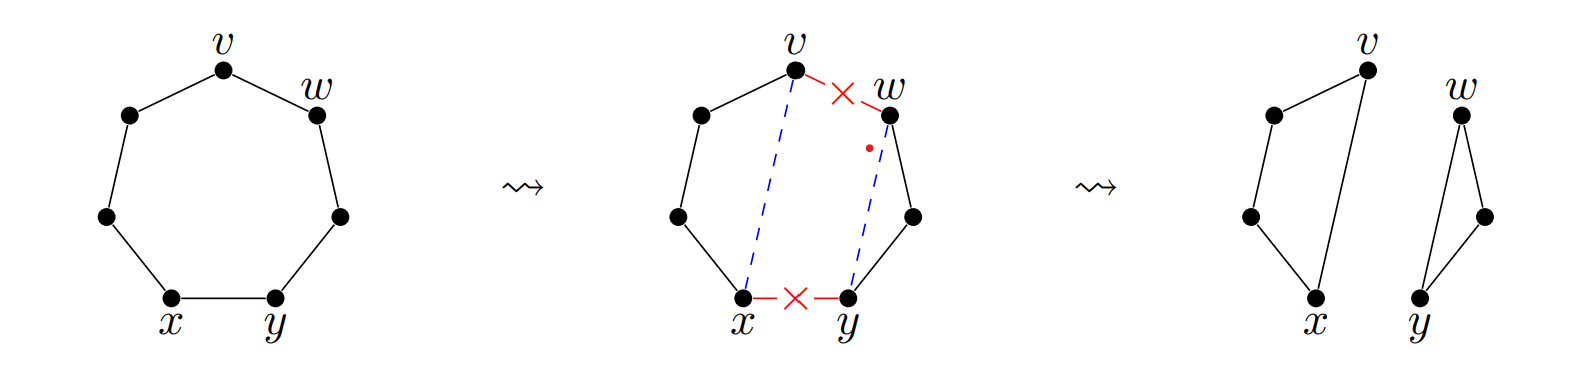
\includegraphics[width=0.8\textwidth]{Edgeswap.png}  
  \end{figure}

  Now, to prove our claim. Say the vertices in decreasing order of degree are $v_1, \dots, v_n$ and $v_1$ has a degree $d$. We need to prove that there's a graph with 
  the given degree sequence, where $v_1$ is connected to every vertex in the set $S = \{v_2, v_3, \dots, v_{d+1}\}$. So let's assume this isn't the case $v_1$ isn't connected
  to $v_i \in S$. Since $v_1$ needs to satisfy its degree requirements, it has to be connected with at least 1 vertex outside $S$, let's say it's connected to $x \notin S$.
  If you think about our goal operation, we already have $3$ vertices ready, $v_1, v_i, x$. We just need a fourth vertex, that $v_i$ is connected to and $x$ isn't connected to.
  But why will some vertex exist? Ok, assume the contrary, there's no such vertex. Every vertex that $v_i$ is connected to, $x$ is also connected to. This would mean that the 
  degree of $x$ is at least as much as the degree of $v_i$. But $x$ is also connected to $v_1$, that $v_i$ isn't connected to, so its degree is strictly more than $v_i$.
  But that's a contradiction, if degree of $x$ is more than $v_i$, it must be in the set $S$ right, as $S$ has all the highest degree vertices. So we can conclude there is 
  some vertex $y$ such that $v_i$ is connected to $y$, but $x$ isn't. And then we can perform our operation, to keep the degree sequence as same, and get a solution where $v_1$ 
  is connected to $v_i$. This operation can be done as many times as we want, to make $v_1$ connected to every vertex of $S$. So we're done.

  \begin{figure}[H]
    \centering
    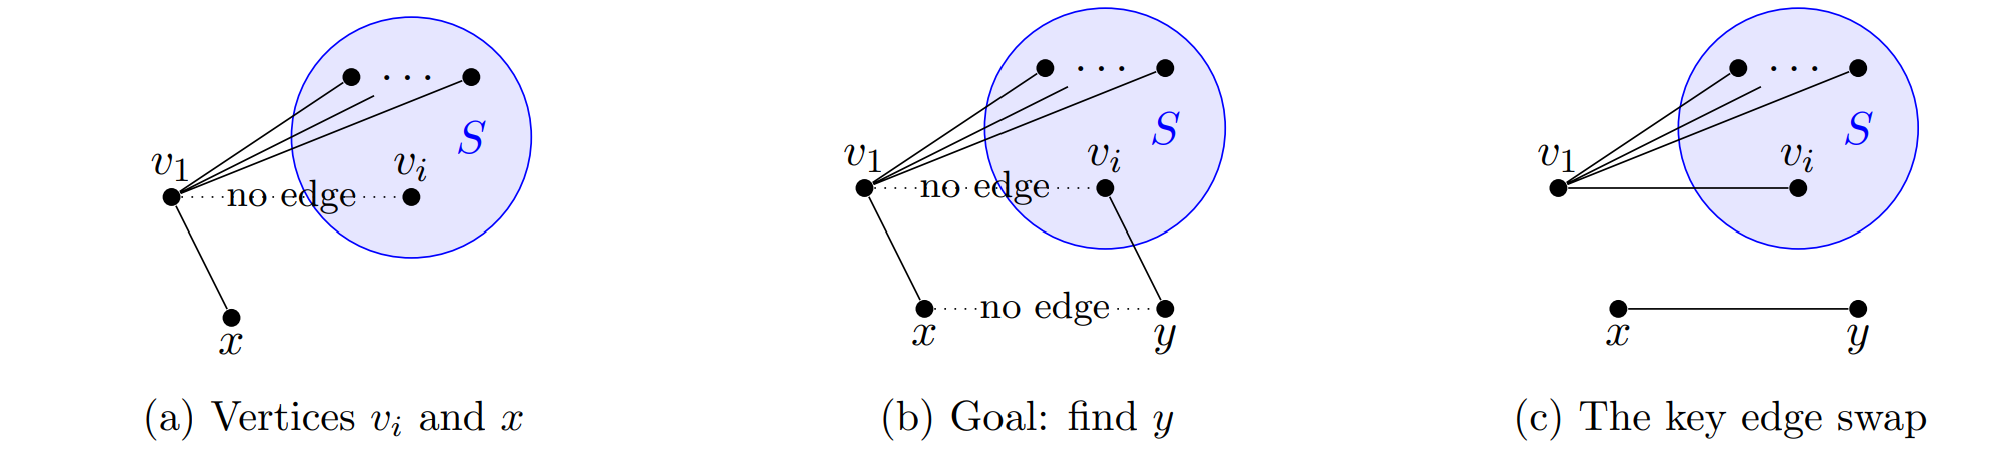
\includegraphics[width=0.8\textwidth]{DegSeqProof.png}  
  \end{figure}
    
  \item Our idea is to sort intervals based on increasing order of end time. The intuition behind this is that, there will be very few people who can show the first person the ad,
  after this sorting, and it is easier to think of some greedy approach. While checking who all arrive before the first person leaves, isn't it best to select the one who leaves
  the latest? This seems intuitive right, as we want most number of people to see the ad.

  Let's prove this claim. Suppose there's some optimal solution where among the people who overlap with the first person, the one with the latest leaving time (call this person $L$)
  isn't selected. So some other person who overlaps with the first guy is selected $K$. Can we always swap this person with the person we claim? One thing to observe is that, $L$ 
  is going to overlap with everyone before $L$ in our array. This is because $L$ arrives before anyone leaves, and leaves only after every single person before $L$ leaves. So everyone
  will see $L$ before leaving. Now for the elements after $L$, is there any person there who $K$ sees but $L$ doesn't see? That's not possible. If they are after $L$ in the array
  they leave way after $K$, so in order for $K$ to see them, they have to arrive before $K$ leaves, but this would mean they also arrive before $L$ leaves, so basically they see $L$ too.
  
  So what have we proven? Anyone $K$ sees, $L$ is going to see, so we might as well pay $L$ instead of $K$. And if we pay $L$, we know for sure we aren't going to pay anyone before $L$
  (same proof as the claim) if we're being optimal. So we continue the same algorithm for the array, starting from after $L$. Note that some intervals after $L$ might have already seen 
  the ad, but that doesn't mean we shouldn't pay them in the optimal solution. Our new first person is going to be the first person who $L$ doesn't see. But the one we select is going to 
  be the one who overlaps with the first person and leaves the latest, this could potentially be someone before the first person, we have to start checking from after $L$ itself.

  If we just apply our claim inductively, we'll be able to prove that our greedy strategy works.

  \item We have $\binom{n}{2}$ pairwise distances. We want to make sure that as many of the small distances as possible aren't from one set to the other, so we try the following greedy 
  approach. First we sort all the pairwise distances in ascending order, and since we don't know which numbers in the same set, assume they are all in different singleton sets for now.
  Now we iterate through the pairwise distances. If suppose the 2 elements are in different sets, we merge them to 1 cluster. We stop our algorithm whenever we have done so much merging that 
  we have only $k$ sets, and we can't do any more merging. Note that there'll be exactly $n-k$ merges.

  We have to prove by induction that every merge we do is valid. But how to phrase this a bit better? At any point in our algorithm, when we detect that $i$ and $j$ are in different clusters, 
  there exists an optimal solution where they are in the same cluster.

  So how do we do this induction? So we assume all the previous merges we have done so far are valid i.e. there exists an optimal solution where elements are in the same cluster, whenever our 
  they are in the same set in our algo. Now we detect 2 new elements which we want to merge. What if there's an optimal solution without these 2 elements in the same set? The spacing of this 
  clustering is at least as big as the distance between these 2 elements, as they are in different sets in the optimal solution. And for the clustering produced by our greedy algo, the spacing
  is at most the distance between these 2 elements, as all the pairwise distances including this distance, and the ones greater than it, don't appear in the spacing term of the greedy algo. Which 
  proves that the greedy algo also outputs some optimal clustering.

  \subsection*{\Large\bfseries Dynamic Programming}

  \subsubsection*{Flavour 1: where the subproblems are on suffixes/prefixes of the input.}

  \item We first sort based on starting time. Now we divide by cases on whether we select the first interval or don't. If we don't, our answer is just going to be the answer for the subarray from
  2 to $n$. If we select the first interval, we have to reject all the intervals which start before the first interval ends. But note that after rejecting everything, we are still going to be left 
  with a contiguous subarray, from some $k$ to $n$, only because the array is sorted by starting time. To find this $k$, we have to just binary search actually. The query is the first interval's 
  end time, and whatever index you get from the binary search, that will decide from which point you have to solve the subproblem. In the end our reucrsion is going to be like
  $f(1, n) = \max(f(2,n), l(I_1)+f(k,n))$. Since by applying this recursion the subarray always ends in $n$, and starting index gets smaller, there are at most $n$ distinct recursive calls. To code this 
  up, we can iterate backwards and find $f(i, n)$ for $i$ from $n$ to 1. Each $f(i, n)$ takes $O(\log n)$ time due to the binary search, so overall the time complexity is still $O(n \log n)$.

  \item I don't know which question they are referring to where we found optimal cost \emoji{grinning-face-with-sweat}
  
  \item Again, split based on whether we select the first interval or don't. If you take the first interval, the best you can do is $w_1 + f(k,n)$, where $k$ is the first interval which starts after
  the first interval ends. And if you don't select the first interval, the answer is just $f(2,n)$. So our recursion changes like: $f(1,n) = \max(f(2, n), w_1 + f(k,n))$. We can iterate backwards 
  to calculate $f(i,n)$ for all $i$, in $O(n \log n)$ time.

  \item It's the same case split again. If we don't select the first interval, the answer is just $f(2,n)$. If we select the first interval, the number of subsets is $f(k,n)$. So the recursion is
  $f(1,n) = f(2,n) + f(k,n)$, where $k$ is the first interval which starts after the first interval ends. 

  \item A natural first idea would be to case split based on which hotel we are staying in for the first night. Let $dp[i]$ be the minimum cost to travel, starting from city $i$. We basically need
  $dp[0]$, treating $A$ as the $0^{th}$ city, and our base case is $dp[n+1] = 0$, treating $B$ as the $(n+1)^{th}$ city. Our recursion is something like this:
  \[ dp[i] = \min_{j \in S_i} (dp[j] + c_j) \text{, $S_i$ is the set of cities which can be reached from city $i$ } \]
  We need some efficient way to calculate $S_i$ for all $i$, while iterating in our algorithm. It's enough to see which is the last city, and its distance which can be reached from every $i$.
  
  We can solve this itself using subproblems. Let's say for city $i$, we have already calculated $j$, the furthest city we can reach, and its distance which is $d_{i+1} + d_{i+2} + \dots + d_j$.
  Now we want to find the furthest city to reach from city $i-1$, so what we do is just add $d_i$ to our distance, assuming we can still reach $j$. If our distance is still not greater than $d$, 
  great, $j$ is still the furthest city. But if it exceeds $i$, keep decrementing $j$, and subtracting $d_j$ from our distance, until the distance doesn't exceed $d$. This is basically a 2 pointer
  method, so it completes in $O(n)$ time overall, for every $i$.

  Now back to our original question. It will be useful if we could just store all the $dp[j] + c[j]$'s in a multiset right, so that we can just find the minimum in $O(\log n)$ time. The idea is 
  to find $dp[i]$ iterating backwards from $n$ to $1$. We concurrently do our subproblem, whenever we decrement $i$, we add $dp[i] + c[i]$ to our multiset. Whenever we decrement $j$, we delete 
  $dp[j] + c[j]$ from our multiset. After doing all the decrementing to $j$ for the particular $i$, we find the minimum of the multiset, and assign that as $dp[i]$. The time complexity of this 
  algorithm overall is $O(n \log n)$ as we have $n$ additions and deletions to our multiset, and well as $n$ minimum queries.
  
  \item For each vertex $i$ from $n$ to $1$, we find the longest path to vertex $n$. Base case is $dp[n] = 0$. Now to get $dp[i]$, we just do $1 + $ the maximum length from every vertex it connects 
  to. This is $O(E)$, where $E$ is the number of edges.

  \item The normal dynamic programming idea is like this: for each element $i$, find the longest increasing subsequence in the array ending at $i$. Suppose this is done for $i$, and we want to 
  do it for $i+1$. We check $arr[i+1]$, and see which all array elements before it that are smaller than it, because we can append $arr[i]$ to any increasing subsequence ending at those. Our recursion
  is going to be $dp[i] = 1 + \max(\{dp[j] \ | \ j \in S_i\})$, where $S_i$ is the set of all $j$ such that $j < i$ and $arr[j] < arr[i]$. The problem with this approach is that $dp[i]$ takes $O(n)$
  time, so this becomes $O(n^2)$.

  We flip the question a bit. For each length $l$, we store the smallest number a subsequence of length $l$ can end in. If in the first $i$ elements there's a subsequence of length 3 ending with 5, 
  there's no point of keeping track of a subsequence of length 3 ending with 10. Further, our array is going to be in increasing order. This is intuitive right, if you have a sequence of length 5
  ending with 10, subsequence with length 4 is going to have a smaller ending number. The fact that the array is sorted could help us do something like binary search.

  Let's say you are in the middle of your iteration, and what you have stored so far is $[2, 3, 5, 9, 10, 12]$ i.e. the smallest ending for a subsequence of length 1 is 2, smallest ending for a subsequence
  of length 2 is 3, and so on. Now let's say the next element of the array you process is 7, how will you update what you are storing? Firstly, 7 can only be appended to sequences of length 1,2,3. There's no
  way we could append to a sequence of length 4,5, or 6, as the smallest ending of a subsequence that long, is already larger than 7. Is there any point appending 7 to a sequence of length 1,2? That creates
  sequence of length 2,3 that end in 7, but we have sequences of that length ending in smaller numbers, so this is useless. So let's append it to a sequence of length 3, this gives a sequence of length 4 ending 
  in 7. This is finally something useful, we have to update the 9 to a 7. From this example, it's clear that only one number has to be updated. For each entry in the input array, find between which 2 numbers
  in our dp array that it lies in, and update the larger number to the input array element. Two edge cases are there though, When our input array element is smaller than our whole dp array, just update the 
  first element. If it's greater than our whole dp array, append the array element to our dp array, as we have a new length of increasing subsequence we can achieve. This algorithm is $O(n \log n)$, as for 
  each element of our input array we take $O(\log n)$ time in binary search.

  \item Let $dp[i]$ represent the solution in the subarray from $i$ to $n$. We iterate backwards, and let's say $dp[i+1]$ to $dp[n]$ are calculated. Now for $dp[i]$, either we select $arr[i]$ or not. If we
  don't select $arr[i]$, the optimal sum is just $dp[i+1]$. If we select $arr[i]$ then we can't select $arr[i+1]$, so we just have to select elements from index $i+2$ to $n$ such that none of them are 
  consecutive. This is just $dp[i+2]$. Finally our recursion is $dp[i] = \max(dp[i+1], arr[i] + dp[i+2])$. This takes $O(n)$ time overall. As we have $n$ $O(1)$ calculations.

  \subsubsection*{Flavour 2: where the subproblem is on a substring of the input.}

  \item We case split based on what't the last multiplication we should do. If we multiply $A_1 A_2 \dots A_i$ with $A_{i+1}$ $A_{i+2} \dots A_n$ last, what's our cost? The first term has dimension $p_1 
  \times p_{i+1}$ and the second term has dimensions $p_{i+1} \times p_{n+1}$ so the cost is $p_1 p_{i+1} p_{n+1}$. We take cases for all $i$, and also, we have the subproblems to solve, how get the 2
  terms most efficiently. Overall our recursion is like this:
  \[dp[1 .. n] = \min_i (dp[1 .. i] + p_1 p_{i+1} p_{n+1} + dp[i+1 .. n]), i \in \{1, 2, \dots, n-1\} \]
  In the recursion, we are always having some contiguous subarray, so there are at most $O(n^2)$ recursive calls. Our base case is that $dp[i .. i] = 0$. Also one more thing in the recursion is that, the 
  size of the subarray we call recursively is strictly decreasing. So to do this algo iteratively, we first store all the solutions for subarray of length 1, length 2, and so on, so that we can directly 
  access solutions of smaller subarrays whenever using the recursive function. Also, each recursive call takes $O(n)$ time, as we have to find the minimum of $O(n)$ number of terms.
  So overall this algo takes $O(n^3)$ time.

  \item We partition cases based on which element is the root of the tree. If $a_k$ is the root, $a_1$ to $a_{k-1}$ have to be in the left subtree, and $a_{k+1}$ to $a_n$ have to be in the right subtree.
  The left and right subtree have to separately be constructed optimally inorder for them for the total tree to be optimal. If the optimal sum for the left subtree alone is $dp[1..k] = \sum f_i d_i$, the 
  contributing factor in the final tree will be $\sum f_i (d_i + 1)$ as each node has extra depth by 1. This simplifies to $\sum f_i d_i + \sum f_i$. A similar story holds for the right subtree. So the
  final recursion is:
  \[dp[1 .. n] = \min_k \left((dp[1 .. (k-1)]) + \sum_{i=1}^{k-1} f_i + f_k + (dp[(k+1) .. n]) + \sum_{k+1}^{n} f_i \right) \] 
  Actually all the summations of $f_i$ can be grouped together, to just summation of all $f_i$'s. So the summation of $f_i$'s are independent of $k$, we can take this term outside.
  \[dp[1 .. n] = \left(\sum_{i=1}^n f_i \right) + \min_k [dp[1 .. (k-1)] + dp[(k+1) .. n]], k \in \{1, 2, \dots, n\} \] 
  it might look like the $\sum f_i$ term will make the time compexity extremely bad, but this is just a sum of frequencies of some contiguous subarray. If we just do a precomputation of prefix sums, it
  becomes very easy to get these values ($O(1)$ time in fact). Again, our recursion only calls contiguous subarrays, so there are $O(n^2)$ recursive calls. For each recursive call, we have to find the maximum
  among $O(n)$ values, which takes $O(n)$ time. So overall, just like the previous question, the time complexity is $O(n^3)$.

  \item Take cases based on which is the first line segment. If the first line segment is from point 1 to point $i$, we just find the best fit line from point 1 to point $i$, add $C$ as we are doing a partition, 
  and then find the optimal solution from point $i$ to point $n$. One edge case is that we don't do any partition i.e. $i = n$ itself, but this is easy to take care of. Our recursion will go like this:
  \[dp[1 .. n] = min (min_i (best\_fit[1 .. i] + C + dp[(i+1) .. n]), best\_fit[1 .. n]) \]
  We are always calling dp from some index to $n$, so there are $O(n)$ recursive calls. For each recursive call, we have to find minimum among some $O(n)$ terms, so overall it looks like this will be $O(n^2)$.
  But there's an issue, the $best\_fit$ terms have to be calculated before hand for each contiguous subarray, so $O(n^2)$ calculations to be done. Each calculation has a closed form solution, which takes $O(n)$
  time to calculate. So overall, the precomputation is $O(n^3)$, so the time complexity is $O(n^3)$.

  \subsubsection*{Flavour 3: where the subproblem has two different parameters.}

  \item We take cases based on if the first letter of $A$ matches with the first letter of $B$. First of all, if their first letters are different, there's no choice to be made. Ignore the first letter of $A$ and
  solve the same question. Suppose $A$, $B$ have the first same letters, there's a choice to be made. Again we could decide not to match, and ignore the first letter of $A$. But we could also choose to match, in 
  which case we incur a cost of $p_1$, and then optimally solve the question for $A$ without its first letter, $B$ without its first letter. If we just keep applying this, we can see that there are only $O(mn)$ 
  recursive calls. Each call is trying to solve matching of $A[i .. m], B[j .. n]$. What are our base cases? If the substring of $B$ has zero length, the answer is $0$. If the substring of $B$ has non zero length
  and the substring of $A$ has zero length, we are stuck, we can't do any matching. So it's like the answer is infinite. Anywhere else, the recursion works. Let $dp(A[i], B[j])$ be the optimal cost of matching 
  $A[i..m], B[j..n]$.
  \begin{align*}
    dp(A[i], B[j]) &= dp(A[i+1], B[j]) \text{ if } A[i] \neq B[j] \text{, else} \\
    dp(A[i], B[j]) &= \min(dp(A[i+1], B[j]), dp(A[i+1], B[j+1]) + p_j)
  \end{align*}
  

  \item Let $dp(i, w)$ be the maximum value you can get from the first $i$ elements when the total weight is bounded by $w$. Our base cases are $dp(i, 0) = 0$, $dp(0, w) = 0$. Now it's a simple case split based
  on if we choose the $i^{th}$ element or not. If in the optimal answer we don't choose it, the answer is just $dp(i-1, n)$. If we do choose it, we now get a value of $v_i$, but rest of the weights can't sum more
  than $w - w_i$. So $dp(i,w) = \max(dp(i-1,w), v_i + dp(i-1, w - w_i))$.

  Now we need some other way of doing the question. Instead of getting the maximum value for particular weights, just get the minimum weight for some particular values. Let $dp(i, v)$ be the minimum weight to get a
  total value of $v$, using the first $i$ elements. The maximum value you can get is just $\sum v_i$, so we have $\sum v_i \times n$ possible recursive calls. Now again take cases based on if you choose the $i^{th}$ 
  element or not. If you don't choose it, your answer is just $dp(i-1, v)$. If you choose it, your answer is $w_i + dp(i-1, v - v_i)$. Our base cases are $dp(i,0) = 0$, as we need 0 weight to get a value of $0$. What
  about $dp(0,v)$, when $v \neq 0$. This is not even possible to achieve, so shouldn't be a case and since we are taking minimum, we can just initialize this to $\infty$. After all these $dp$ values are calculated,
  we should find the maximum $v$ such that $dp(n,v) \leq W$.

  \subsubsection*{Flavour 4: where subproblems are parameterized by a prefix and something more}

  \item Let $dp_A(i)$ and $dp_B(i)$ be the maximum earning you can get from the beginning of day $i$, starting at city $A$, $B$ respectively. Our base cases are $dp_A(n) = a_n$, and $dp_B(n) = b_n$. To find $dp_A(i)$,
  there are 2 choices. Either you stay in city A, and get the earning $a_i$, and from then onwards it is $dp_A(i+1)$. Or you decide to pack up and leave, you don't get any earnings on day $i$, incur a cost of $c$, and
  from then onwards it is $dp_B(i+1)$. So the recursion is $dp_A(i) = \max(dp_A(i+1) + a_i, dp_B(i+1) - c)$. Similarly, $dp_B(i) = \max(dp_B(i+1) + b_i, dp_A(i+1) - c)$. So we iterate backwards and calculate $dp_A(i),
  dp_B(i)$ for all $i$. Our final answer is just $\max(dp_A(1), dp_B(1))$.

  \item Done in Q20
  
  \item We take cases on which index $b_1$ is paired with. Firstly, it can't be paired with $b_2$ to $b_5$ based on the constraint. Check which of $b_6$ to $b_n$ it can be paired with. If it is paired with some $b_i$, the 
  sequence is split into 2 parts: $b_2$ to $b_{i-1}$, and $b_{i+1}$ to $b_n$. None of the letters can be paired from one of these sequences to the other, because of the non-crossing condition. So all we have to do is solve
  the problem recursively for each of these subarrays. Another corner case is when $b_1$ is paired with nothing, in which case our answer is the subproblem solved from $b_2$ to $b_n$. Our recursion is like this:
  \[dp[1 .. n] = \max(1 + \max_i (dp[2 .. (i-1)] + dp[(i+1) .. n]), dp[2 .. n]) \]
  $i$ belongs to some set where pairing with the first element is possible, and $i > 5$. Since each recursive call is on a subarray, there are $O(n^2)$ recursive calls, and each recursive call takes $O(n)$ time to compute.
  So this algo is $O(n^3)$, and our base cases for the recursion are when the subarray length is $\leq$ 5, the number of pairings is 0.

  \item
 
  \item
  
  \item For each node, we are maintaining what is the shortest path length to the destination. You just also need to maintain which node to go next, at each node. Whenever you compute minimum among which nodes to go next,
  just store the node which gives you minimum. After the whole algo, we can just move along this path to get the optimal path.

  \item Bellman Ford will just give you the optimal path of length at most $n-1$, this won't be the optimum path if there are negative weight cycles. The idea to detect negative cycles is like the following. Add a sink
  vertex i.e. add a new vertex such that every vertex has a directed edge of weight 0 to it. If there's any negative cycle, there's also a path going through this cycle and ends up at the sink, since you can go from any node to the sink.
  For any node in this cycle, the minimum weight path to the sink is $-\infty$, as you can just pump this cycle as many times as you want. Using this as motivation, our idea is like this: check if $opt(n,v) = opt(n-1,v)$
  for all nodes $v$ (where $opt(n,v)$ is the minimum weight path of length atmost $n$ from $v$ to the sink). If the graph has no negative weight cycles, obviously $opt(n,v) = opt(n-1,v)$ as paths of length greater than $n-1$
  will have cycles, and won't be optimal. The converse is also true, assume $opt(n,v) = opt(n-1,v)$ for all nodes $v$. This means that the optimal solution at each node doesn't change. Then if we do one more iteration of Bellman Ford,
  $opt(n+2, v) = opt(n+1, v)$ for all $v$. We have basically reached a stable point in our algorithm. But this can never happen for a graph with negative weight cycles, as for some vertex, $opt(n,v)$ should blow up (or down) to 
  $-\infty$ as we said before. So a quick way if-and-only-if way to check if there are negative weight cycles, is to see if $\forall v \ opt(n,v) = opt(n-1,v)$.

  \end{enumerate}
\end{document}